%
% 1-beispiele.tex %% Beispiele partieller Differentialgleichungen
%
% (c) 2008 Prof Dr Andreas Mueller
%
\chapter{Geometrie PDGLen erster Ordnung\label{chapter-geometrie}}
Bei gew"ohnlichen Differentialgleichungen kann man sich ein grobes
Bild des Verlaufs der L"osungen dadurch verschaffen, dass man
die von der Differentialgleichung vorgegeben Steigung der L"osungskurve
in jedem Punkt als Richtungsfeld aufzeichnet. Ein geometrisches
Bild erlaubt den L"osungsverlauf abzusch"atzen. Die L"osung einer
partiellen Differentialgleichung ist eine Funktion von mehreren Variablen,
bei zwei Variablen k"onnen wir den Graphen dieser Funktion als Fl"ache
"uber dier $x$-$y$-Ebene visualisieren. Wie l"asst sich der Begriff der
Steigung "ubersetzen?

\section{Kurven auf der L"osungsfl"ache}
\rhead{Kurven auf der L"osungsfl"ache}
\subsection{Allgmeine PDGL erster Ordnung}
Als Beispiel betrachten wir die folgende partielle Differentialgleichung
erster Ordnung f"ur die Funktion $u(x,y)$
$$
F\biggl(x,y,u(x,y),\frac{\partial u}{\partial x},\frac{\partial u}{\partial y}\biggr)=0.
$$
Diese Gleichung beschreibt einen impliziten Zusammenhang zwischen
dem Ort im $x$-$y$-$u$-Koordinatensystem und den beiden Steigungen
$\partial_xu$ und $\partial_yu$.

Ein Anfangswertproblem, bei dem die Anfangswerte f"ur $x=0$ als
Funktion $g(y)$ festgelegt sind, $u(0,y)=g(y)$, legt auch die
partiellen Ableitungen $\partial_y u(0,y)=g'(y)$ fest.  Die partielle
Differentialgleichung schr"ankt damit ein, welche m"oglichen Ableitungen
$\partial_xu(0,y)$ m"oglich sein. Oft wird dies nicht eindeutig sein,
die Steigung in $x$-Richtung kann also verschiedene Werte annehmen,
es kann verschiedene L"osungsfunktionen geben. "Ahnlich wie bei der
L"osung gew"ohnlicher Differentialgleichungen ist zu jedem Wert
aus der bereits bekannten partiellen Ableitung $\partial_yu(x,y)$
die Steigung $\partial_xu(x,y)$ bestimmt, es ist somit plausibel, dass
sich die L"osung "ahnlich wie bei der L"osung gew"ohnlicher Differentialgleichungen
entwickeln l"asst. In voller Allgmeinheit ist dies nicht ganz einfach,
und f"ur unsere Zwecke auch nicht notwendig, denn alle wesentlichen
Eigenschaften lassen sich an dem einfacheren Fall der quasilinearen
PDGL auch beobachten.

\subsection{Quasilineare PDGL erster Ordnung}
F"ur eine quasilineare PDGL erster Ordnung
$$
a\frac{\partial u}{\partial x}
+
b\frac{\partial u}{\partial y}
=
c
$$
kann man immer dann, wenn mindestens einer der Koeffizienten
$a(x,y,u)$ und $b(x,y,u)$ von $0$ verschieden ist, die Gleichung
nach einer der partiellen Ableitungen aufl"osen. Die eine partielle
Ableitung legt also die andere fest. Am Anfang ist die eine partielle
Ableitung durch die Anfangswerte festgelegt, also steht auch schon fest,
mit welcher Normalableitung sich die L"osung weiter entwickeln wird.
Wir erwarten daher, dass sich quasilineare PDGL besonders leicht
l"osen lassen.

Die L"osung wird durch die folgende Beobachtung vereinfacht.
Die PDGL kann auch als Vektorgleichung geschrieben werden:
$$\begin{pmatrix}a\\b\\c\end{pmatrix}
\cdot
\begin{pmatrix}
\frac{\partial u}{\partial x}\\
\frac{\partial u}{\partial y}\\
-1
\end{pmatrix}=0.
$$
Der zweite Vektor ist die Normale auf den Graphen der Funktion
$z=u(x,y)$, die Gleichung sagt also, dass diese Normale senkrecht
auf dem Vektor $(a,b,c)$ steht. Insbesondere ist $(a,b,c)$ auf
jeden Fall tangential an die Fl"ache.

Somit haben wir ein Vektorfeld gewonnen, welches in jedem Punkt tangential
an die gesuchte Fl"ache verl"auft. Ist ein Punkt der Fl"ache bekannt,
kann man davon ausgehend eine L"osungskurve des Vektorfeldes konstruieren,
die die Fl"ache nicht verl"asst. Diese Kurven heissen Charakteristiken der PDGL.

Damit l"asst sich das Cauchy-Problem l"osen. Die Vorgabe einer Anfangsbedingung
legt ja genau ein Menge von Punkten fest, durch die die L"osungsfl"ache
verlaufen soll. Von jedem Punkt der Anfangsbedingung aus kann man also
eine L"osungskurve des Vektorfeldes konstruieren, diese Schar von L"osungskurven
bildet dann die gesuchte L"osungsfl"ache.

Sind die Koeffizienten der Differentialgleichung differenzierbare Funktionen,
dann ist das Vektorfeld differenzierbar.
Ist auch die Anfangsbedingung differenzierbar,
dann besagen die allgemeinen S"atze "uber die Abh"angigkeit der L"osung einer
gew"ohnlichen Differentialgleichung von den Anfangsbedingungen, dass die so
konstruierte L"osungsfl"ache differenzierbar ist.

Insgesamt haben wir damit das Problem der L"osung der PDGL auf das Problem 
zur"uckgef"uhrt, beliebige L"osungskurven eines Vektorfeldes, also auf
eine gew"ohnliche Differentialgleichung zur"uckgef"uhrt.


\section{Beispiele}
\subsection{Konstante Koeffizienten\label{konstantekoeff}}
Wir betrachten die Differentialgleichung
$$
\frac{\partial u}{\partial x}+2\frac{\partial u}{\partial y}=3
$$
mit der Anfangsbedingung $u(0,y)=\sin y$ und m"ochten eine L"osung f"ur
$x>0$ finden.

Das konstante Vektorfeld $\begin{pmatrix}1&2&3\end{pmatrix}^t$ hat die
L"osungskurven
$$
t\mapsto\begin{pmatrix}x_0\\y_0\\z_0\end{pmatrix}+t\begin{pmatrix}1\\2\\3\end{pmatrix}
$$
Der Anfangspunkt $(0,y_0,\sin y_0)$ entwickelt sich also mit der Zeit zu
$$
\begin{pmatrix}0\\y_0\\\sin y_0\end{pmatrix}+t\begin{pmatrix}1\\2\\3\end{pmatrix}
=
\begin{pmatrix}
t\\
y_0+2t\\
\sin y_0+3t
\end{pmatrix}.
$$
Diese Kurvenschar beschreibt die L"osungsfl"ache, wir m"ochten daraus aber
wieder die L"osung in der vertrauteren Form $u(x,y)$ gewinnen. Wir m"ussen
also herausfinden, welcher Anfangspunkt $(0,y_0)$ auf der $y$-Achse sich
zu $(x,y)$ entwickeln wird. Dazu muss man $t$ und $y_0$ so finden, dass
$$
\begin{pmatrix}
t\\
y_0+2t
\end{pmatrix}
=
\begin{pmatrix}
x\\y
\end{pmatrix}
\quad
\Rightarrow
\quad
t=x\text{ und } y_0+2t=y \Rightarrow y_0=y-2x
$$
Da jetzt $y_0$ und $t$ durch $x$ und $y$ ausgedr"uckt sind, k"onnen wir
$u(x,y)$ durch Einsetzen berechnen:
$$
u(x,y)=\sin y_0+3t=\sin(y-2x)+3x.
$$

\subsection{Kreisf"ormige Charakteristiken}
Wir l"osen die Differentialgleichung
$$
y\frac{\partial u}{\partial x}-x\frac{\partial u}{\partial y}=0
$$
Gem"ass der Methode der Charakteristiken m"ussen wir die L"osungskurven
des Vektorfeldes
$$
\begin{pmatrix}
y\\-x\\0
\end{pmatrix}
$$
finden. Da die $z$-Komponente verschwindet, sind die $z$-Komponenten
der L"osungskurven konstant, wir ignorieren sie daher in der nachstehenden
Rechnung.

L"osungen f"ur das Vektorfeld 
$$
\begin{pmatrix}
y\\-x
\end{pmatrix}
$$
in der Ebene sind Funktionen $x(t)$ und $y(t)$, welche die Gleichungen
\begin{align*}
\dot x(t)&=y(t)\\
\dot y(t)&=-x(t)
\end{align*}
erf"ullen. Leitet man die erste Gleichung ab, und setzt die zweite
darin ein, erh"alt man die Differentialgleichung zweiter Ordnung
$$
\ddot x(t)=-x(t)
$$
mit den bekannten L"osungen $a\cos t$ und $a \sin t$. Da die L"osungskurve
zur Zeit $t=0$ auf der $y$-Achse beginnen soll, muss sie in Vektorschreibweise
$$
\begin{pmatrix}
x(t)\\y(t)
\end{pmatrix}
=y_0\begin{pmatrix}
\sin t\\
\cos t
\end{pmatrix}
$$
sein, die Kurven sind also Kreise mit Radius $y_0$ um den Nullpunkt. Offenbar
k"onnen wir jeden Punkt der Ebene von einem Punkt in der Halbgeraden
$\{(0,y_0)|y_0 <0\}$ aus erreichen, die Anfangsbedingung muss also nur f"ur
$y_0<0$ spezifiziert werden.

Die L"osung zur Anfangsbedingung $g(y)$ kann jetzt wie folgt bestimmt werden.
Zu einem Punkt $(x,y)$ m"ussen $y_0$ und $t$ gefunden werden, davon brauchen wir
jedoch nur den Betrag, also $y_0=-\sqrt{x^2+y^2}$. Die L"osung ist also
$$
u(x,y)=g(-\sqrt{x^2+y^2}).
$$

Aus diesem Beispiel k"onnen wir mehrere Lehren ziehen: 
\begin{enumerate}
\item Dass Festlegung einer Anfangsbedingung f"ur $y_0>0$ nicht n"otig ist,
kann man der Differentialgleichung in unmittelbarer N"ahe der $y$-Achse nicht
ansehen, erst der Verlauf der Charakterisitiken im Grossen erm"oglicht
diese Erkenntnis. Dieses Ph"anomen wird durch den ``zus"atzlichen Platz''
erm"oglicht, den der zweidimensionale Definitionsbereich der PDGL gegen"uber dem
eindimensionalen Definitionsbereich der gew"ohnlichen DGL bietet.
\item Der Punkt $(0,0)$ hat spezielle Eigenschaften: wenn die L"osung stetig
sein soll, muss $g(0)=\lim_{y\to 0-} g(y)$ sein. Damit die L"osung differenzierbar
wird, muss aber zus"atzlich $g'(x)=0$ sein.
\end{enumerate}

\subsection{Ein nicht l"osbares Anfangswertproblem\label{unloesbar}}
Die Differentialgleichung
$$
x\frac{\partial u}{\partial x}
+
y\frac{\partial u}{\partial y}
=0
$$
soll zu den Anfangsbedingungen $u(0,y)=\sin y$ gel"ost werden.
Dazu berechnen wir wieder zuerst die Charakteristiken (ohne die 
$z$-Komponente, die wieder konstant ist)
$$
\frac{d}{dt}
\begin{pmatrix}
x(t)\\y(t)
\end{pmatrix}
=
\begin{pmatrix}
x(t)\\y(t)
\end{pmatrix}
\quad
\Rightarrow
\quad
\left\{
\begin{aligned}
\dot x(t)&=x(t)\\
\dot y(t)&=y(t)
\end{aligned}
\right.
$$
Die L"osungskurven sind Strahlen durch den Ursprung:
$$
\begin{pmatrix}
x(t)\\y(t)
\end{pmatrix}
=\begin{pmatrix}x_0\\y_0\end{pmatrix}e^t
$$
Um die L"osung zu konstruieren, m"ussen wir jetzt zu einem Punkt
$(x,y)$ den Anfangspunkt der zugeh"origen Charakteristik auf der $y$-Achse
finden. Da alle Charakteristiken durch den Nullpunkt gehen, ist dies 
gar nicht m"oglich. 

Das Problem r"uhrt daher, dass wir die Anfangsbedinung selbst auf einer
Charakteristik festgelegt haben, die Charakteristiken sind also als
Anfangskurven ungeeignet. Nur wenn die Anfangsbedingung auf einer Kurve
festgelegt wird, die transversal, also nirgends tangential, zu den
Charakteristiken verl"auft, kann das Anfangswertproblem gel"ost werden.

\section{Allgemeines Verfahren}
Eine Differentialgleichung der Form
$$
a(x,y,u)\frac{\partial u}{\partial x}+b(x,y,u)\frac{\partial u}{\partial z}=c(x,y,u)
$$
mit Anfangswerten auf einer Kurve $\gamma$ wird wie folgt gel"ost.

Zu jedem Punkt der Kurve $\gamma$ wird die von diesem Punkt ausgehende
Integralkurve des Vektorfeldes
$$
\begin{pmatrix}
a(x,y,z)\\
b(x,y,z)\\
c(x,y,z)\\
\end{pmatrix}
$$
ermittelt. Die Integralkurve ist L"osung der Differentialgleichung
\[
\frac{d}{dt}
\begin{pmatrix}x(t)\\y(t)\\z(t)\end{pmatrix}
=
\begin{pmatrix}
a(x(t),y(t),z(t))\\
b(x(t),y(t),z(t))\\
c(x(t),y(t),z(t))
\end{pmatrix},
\qquad
\text{Anfangsbedingung:}\;
\begin{pmatrix}x(0)\\y(0)\\z(0)\end{pmatrix}
=\gamma(s),
\]
zu jedem Wert des Kurvenparameters $s$ gibt es so eine Kurve.
Die von dieser Kurvenschar gebildete Fl"ache ist die L"osungsfl"ache
der Differentialgleichung.

Die L"osungskurven h"angen nat"urlich von $s$ ab, wir k"onnen die
Kurvenschar also auch in der Form
$$
\begin{pmatrix}
x(t,s)\\
y(t,s)\\
z(t,s)
\end{pmatrix}
$$
schreiben.
Um die L"osung in der Form $u(x,y)$ anzugeben, muss also die Funktion
$$
(t,s)\mapsto (x(t,s),y(t,s))
$$
invertiert werden, wir m"ussen zu einem Punkt $(x,y)$ die Parameterwerte
f"ur $s$ (welche Kurve) und $t$ (wo auf der Kurve) ermitteln, um dann
mit Hilfe von $z(t,s)$ den Funktionswert an der Stelle $(x,y)$
angeben zu k"onnen.
Ist $(x,y)\to (t(x,y),s(x,y))$ die Umkehrabbildung, dann
ist die L"osung der PDGL:
$$
u(x,y)=z(t(x,y),s(x,y)).
$$

\section{Entstehung von Singularit"aten}
Die L"osung einer partiellen Differentialgleichung h"angt entscheidend
vom Verlauf der Charakteristiken ab. Treffen sich die zwei Charakteristiken
in einem Punkt, ist die L"osung nicht eindeutig bestimmt. Die L"osung
ist also nur solange bestimmt, als sich die Charakteristiken nicht "uberschneiden.
Andernfalls treten Singularit"aten in der L"osung auf.

Als Beispiel betrachten wir die nichtlineare Gleichung 
\begin{equation}
\frac{\partial u}{\partial t}+u\frac{\partial u}{\partial x}=0.
\label{wellenichtlinear}
\end{equation}
mit der Anfangsbedingung 
$$
u(0,x_0)=g(x_0)=e^{-4(x_0-\frac12)^2}.
$$
Nach der Methode der Charakterisitiken brauchen wir eine L"osungskurve
des Vektorfeldes
$$
\begin{pmatrix}
1\\
u\\
0
\end{pmatrix}
$$
durch den Punkt $(0,x_0, z_0)$, also eine L"osung des Differentialgleichungssystems
$$
\left.
\begin{aligned}
\frac{d}{d\tau} t(\tau)&=1\\
\frac{d}{d\tau} x(\tau)&=z(\tau)\\
\frac{d}{d\tau} z(\tau)&=0
\end{aligned}
\quad
\right\}
\qquad
\Rightarrow
\qquad
\left\{
\quad
\begin{aligned}
t(\tau)&=\tau\\
z(\tau)&=z(0)\\
x(\tau)&=z(0)\tau +x(0)
\end{aligned}
\right.
$$
Der Parameter $\tau$ hat also die Bedeutung von $t$.
Die L"osungsfl"ache ist somit
$$
(t,x_0)\mapsto
\begin{pmatrix}
t\\
g(x_0)t+x_0\\
g(x_0)
\end{pmatrix}.
$$
Die Charakteristiken in der $x$-$y$-Ebene sind Geraden mit einer
Steigung, die von $g(x_0)$ abh"angt. Je gr"osser $g(x_0)$ ist, desto
``schneller'' bewegt sich die Integralkurve nach ``rechts''. Grosse
Werte der Anfangsbedingung k"onnen also die kleinen Wert "uberholen,
dabei entsteht eine Singularit"at.

Zur Zeit $t$ hat die L"osungsfunktion die Parameterdarstellung
$$
x_0\mapsto (g(x_0)t+x_0,g(x_0))
$$
die Graphen in Abbildung~\ref{g} zeigen, wie sich die L"osungskurve
mit zunehmender Zeit entwickelt.
Es ist offensichtlich, dass f"ur gen"ugend grosse Zeit $t$ die
L"osungsfl"ache nicht mehr als Graph einer Funktion $u(t,x)$ derstellbar ist.
\begin{figure}
\begin{center}
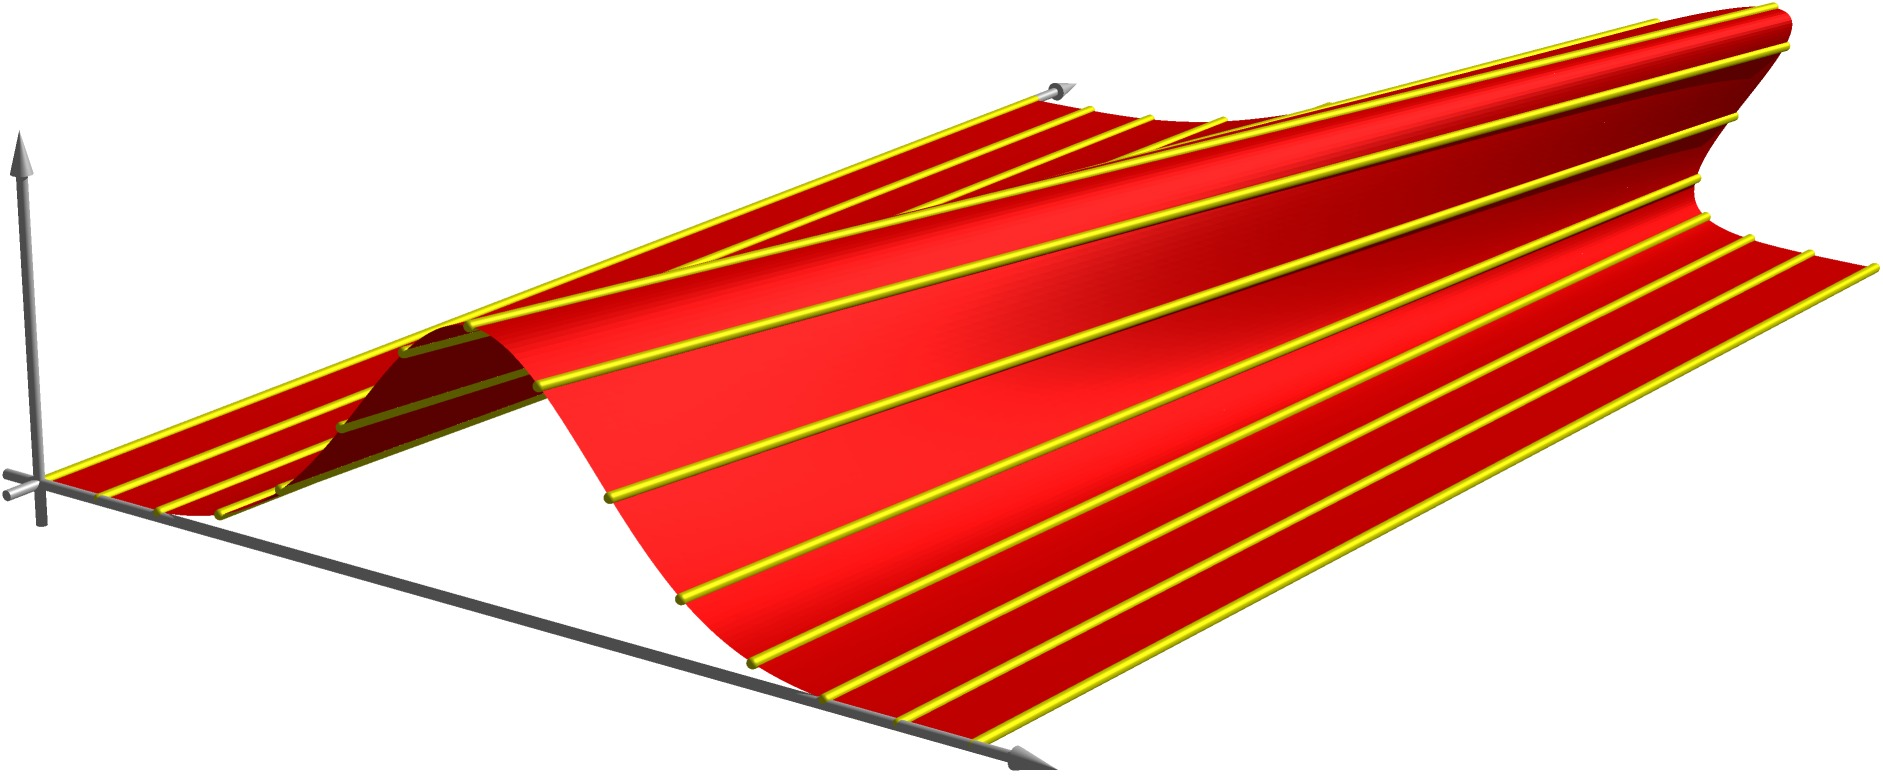
\includegraphics[width=\hsize]{graphics/welle}
\end{center}
\caption{L"osung der Differentialgleichung \ref{wellenichtlinear} mit
entstehender Singularit"at\label{g}}
\end{figure}

\section{Randbedingungen}
Die Methode der Charakterisitiken erlaubt uns herauszufinden, auf welchen
Teilen des Randes die Werte einer L"osunge einer partiellen
Differentialgleichung vorgegeben werden m"ussen.
Die L"osungsfl"ache $u(x,y)$ besteht ja aus Charatkeristiken, sie ist also
genau dann vollst"andig bestimmt, wenn jede Charakteristik durch mindestens 
einen vorgegebenen Randpunkt verl"auft.

F"ur die Differentialgleichung
\[
\frac{\partial u}{\partial x}+2\frac{\partial u}{\partial y}=3
\]
hatten wir die Charakterisiken 
\[
t\mapsto\begin{pmatrix}x_0\\y_0\\z_0\end{pmatrix}+t\begin{pmatrix}1\\2\\3\end{pmatrix}
\]
gefunden. Eine L"osungsfunktion $u(x,y)$ muss von Charakteristiken
"uberdeckt werden. 
Die Projektionen dieser Kurven in die $x$-$y$-Ebene sind Geraden
mit Steigung $2$. Der Rand des Gebietes $\Omega$, in dem die Gleichung gel"ost
werden soll, muss also jede Gerade mit Steigung $2$ h"ochstens einmal
schneiden.

Das Gebiet $\{(x,y)\in\mathbb R^2\,|\, x >0\}$  aus \ref{konstantekoeff}
hat die $x$-Achse als Rand, und diese schneidet jeder Gerade mit Steigung
$2$ genau einmal.
